
% documentclass options:
% ngerman is needed for hyphenation if the thesis contains parts written in German
% BCOR is binding correction
% if you'd rather have a one sided thesis, add `onside' to the documentclass
\documentclass[openany, 11pt, a4paper, BCOR=10mm, english, ngerman]{scrbook}

% include all packages and define commands in setup.tex

%------------------------------------------------------------------------------
%       package includes
%------------------------------------------------------------------------------
    % font encoding is set up for pdflatex, for other environments see
    % http://tex.stackexchange.com/questions/44694/fontenc-vs-inputenc
    \usepackage[T1]{fontenc}  % 8-bit fonts, improves handling of hyphenations
    \usepackage[utf8x]{inputenc}
    % provides `old' commands for table of contents. Eases the ability to switch
    % between book and scrbook
    \usepackage{scrhack}


    % ------------------- layout, default -------------------
    % adjust the style of float's captions, separated from text to improve readabilty
    \usepackage[labelfont=bf, labelsep=colon, format=hang, textfont=singlespacing]{caption}
    \usepackage{chngcntr}  % continuous numbering of figures/tables over chapters
    \counterwithout{equation}{chapter}
    \counterwithout{figure}{chapter}
    \counterwithout{table}{chapter}

    % Uncomment the following line if you switch from scrbook to book
    % and comment the setkomafont line
    %\usepackage{titlesec}  % remove "Chapter" from the chapter title
    %\titleformat{\chapter}[hang]{\bfseries\huge}{\thechapter}{2pc}{\huge}
    \setkomafont{chapter}{\normalfont\bfseries\huge}

    \usepackage{setspace}  % Line spacing
    \onehalfspacing
    % \doublespacing  % uncomment for double spacing, e.g. for annotations in correction

    % ------------------- functional, default-------------------
    \usepackage[dvipsnames]{xcolor}  % more colors
    \usepackage{array}  % custom format per column in table - needed on the title page
    \usepackage{graphicx}  % include graphics
    \usepackage{subfig}  % divide figure, e.g. 1(a), 1(b)...
    \usepackage{amsmath}  % |
    \usepackage{amsthm}   % | math, bmatrix etc
    \usepackage{amsfonts} % |
    \usepackage{calc}  % calculate within LaTeX
    \usepackage[unicode=true,bookmarks=true,bookmarksnumbered=true,
                bookmarksopen=true,bookmarksopenlevel=1,breaklinks=false,
                pdfborder={0 0 0},backref=false,colorlinks=false]{hyperref}


    %==========================================
    % You might not need the following packages, I only included them as they
    % are needed for the example floats
    % ------------------- functional, custom -------------------
    \usepackage{algorithm,algpseudocode}
    \usepackage{bm}  % bold greek variables (boldmath)
    \usepackage{tikz}
    \usetikzlibrary{positioning}  % use: above left of, etc

    % Improves general appearance of the text
    \usepackage[protrusion=true,expansion=true, kerning]{microtype}

%------------------------------------------------------------------------------
%       (re)new commands / settings
%------------------------------------------------------------------------------
    % ----------------- referencing ----------------
    \newcommand{\secref}[1]{Section~\ref{#1}}
    \newcommand{\chapref}[1]{Chapter~\ref{#1}}
    \renewcommand{\eqref}[1]{Equation~(\ref{#1})}
    \newcommand{\figref}[1]{Figure~\ref{#1}}
    \newcommand{\tabref}[1]{Table~\ref{#1}}

    % ------------------- colors -------------------
    \definecolor{darkgreen}{rgb}{0.0, 0.5, 0.0}
    % Colors of the Albert Ludwigs University as in
    % https://www.zuv.uni-freiburg.de/service/cd/cd-manual/farbwelt
    \definecolor{UniBlue}{RGB}{0, 74, 153}
    \definecolor{UniRed}{RGB}{193, 0, 42}
    \definecolor{UniGrey}{RGB}{154, 155, 156}


    % ------------------- layout -------------------
    % prevents floating objects from being placed ahead of their section
    \let\mySection\section\renewcommand{\section}{\suppressfloats[t]\mySection}
    \let\mySubSection\subsection\renewcommand{\subsection}{\suppressfloats[t]\mySubSection}


    % ------------------- marker commands -------------------
    % ToDo command
    \newcommand{\todo}[1]{\textbf{\textcolor{red}{(TODO: #1)}}}
    \newcommand{\extend}[1]{\textbf{\textcolor{darkgreen}{(EXTEND: #1)}}}
    % Lighter color to note down quick drafts
    \newcommand{\draft}[1]{\textbf{\textcolor{NavyBlue}{(DRAFT: #1)}}}


    % ------------------- math formatting commands -------------------
    % define vectors to be bold instead of using an arrow
    \renewcommand{\vec}[1]{\mathbf{#1}}
    \newcommand{\mat}[1]{\mathbf{#1}}
    % tag equation with name
    \newcommand{\eqname}[1]{\tag*{#1}}


    % ------------------- pdf settings -------------------
    % ADAPT THIS
    \hypersetup{pdftitle={Breaking Enigma},
                pdfauthor={Kaleb Davis, Courtney McGorrill},
                pdfsubject={Codes and Ciphers Research Paper},
                pdfkeywords={codes, cryptography, enigma, world war two},
                pdfpagelayout=OneColumn, pdfnewwindow=true, pdfstartview=XYZ, plainpages=false}


    %==========================================
    % You might not need the following commands, I only included them as they
    % are needed for the example floats

    % ------------------- Tikz styles -------------------
    \tikzset{>=latex}  % arrow style


    % ------------------- algorithm ---------------------
    % Command to align comments in algorithm
    \newcommand{\alignedComment}[1]{\Comment{\parbox[t]{.35\linewidth}{#1}}}
    % define a foreach command in algorithms
    \algnewcommand\algorithmicforeach{\textbf{foreach}}
    \algdef{S}[FOR]{ForEach}[1]{\algorithmicforeach\ #1\ \algorithmicdo}

    \usepackage{fancyvrb}
    \newenvironment{CVerbatim}
      {\singlespacing\center\BVerbatim}
      {\endBVerbatim\endcenter} 


\begin{document}
    \pagestyle{empty} % no header and no page number
    % disable hyper links to remove warning "destination with same identifier"
    % this means within this section nothing can be referenced with a hyperlink
    \hypersetup{pageanchor=false}
    
\begin{titlepage}
\begin{center}

\newcommand{\HorizontalLine}{\rule{\linewidth}{0.3mm}}


% _____________________________________________________________________________
\HorizontalLine \\[0.4cm]
\begin{spacing}{3}
    {\huge \bfseries Breaking Enigma}\\
    {\huge \bfseries Codebreaking Techniques from WWII}\\
\end{spacing}
\HorizontalLine \\[1.5cm]
% _____________________________________________________________________________


\vfill  % move the following text to the bottom

\Large {
    Kaleb Davis\\
    Courtney McGorrill\\
    May 2017
}
\end{center}
\end{titlepage}

    \pagestyle{plain} % remove chapter name from top, page number at the bottom

    \mainmatter  % Arabic page numbers
    \chapter{Introduction}\label{chap:introduction}

\todo{Add introduction content}

    \chapter{History}\label{chap:history}

In the first World War, war radios began to have an increasingly large role in military communications. The greatest advantage was the increased range of distance from which one could communicate, but the greatest disadvantage was that messages were easily intercepted. This lead to cipher systems to be developed, but the complexity had to be limited. Cipher clerks were not cryptanalysts or mathematicians. If the system used to encipher a message was too complex, there was an increasingly high risk of error in the message which could have had disastrous consequences in wartime. After the war, it was decided, in multiple countries, that the best way to encipher the messages was to have a user-friendly machine that would increase the complexity of encipherment, while decreasing the complexity of the tasks done by the cipher clerk. In the early 1920’s a German man, Arthur Sherbius, developed Enigma for this very purpose. Enigma was an iteration on several difference cipher machines that centered around using a large number of substitution alphabets, where no single alphabet would repeat until thousands of letters had been processed. The first Enigma was based on several main components: a twenty-six letter keyboard, twenty-six lamps to illuminate the ciphertext, a power supply, three removable wired wheels that rotate on a common axis, a fixed wired reflector, and a fixed wired entry wheel\cite{rfc01}. Future iterations of Enigma would include a plug board where one could essentially swap two characters.

\begin{figure}[h!]
\begin{centering}
  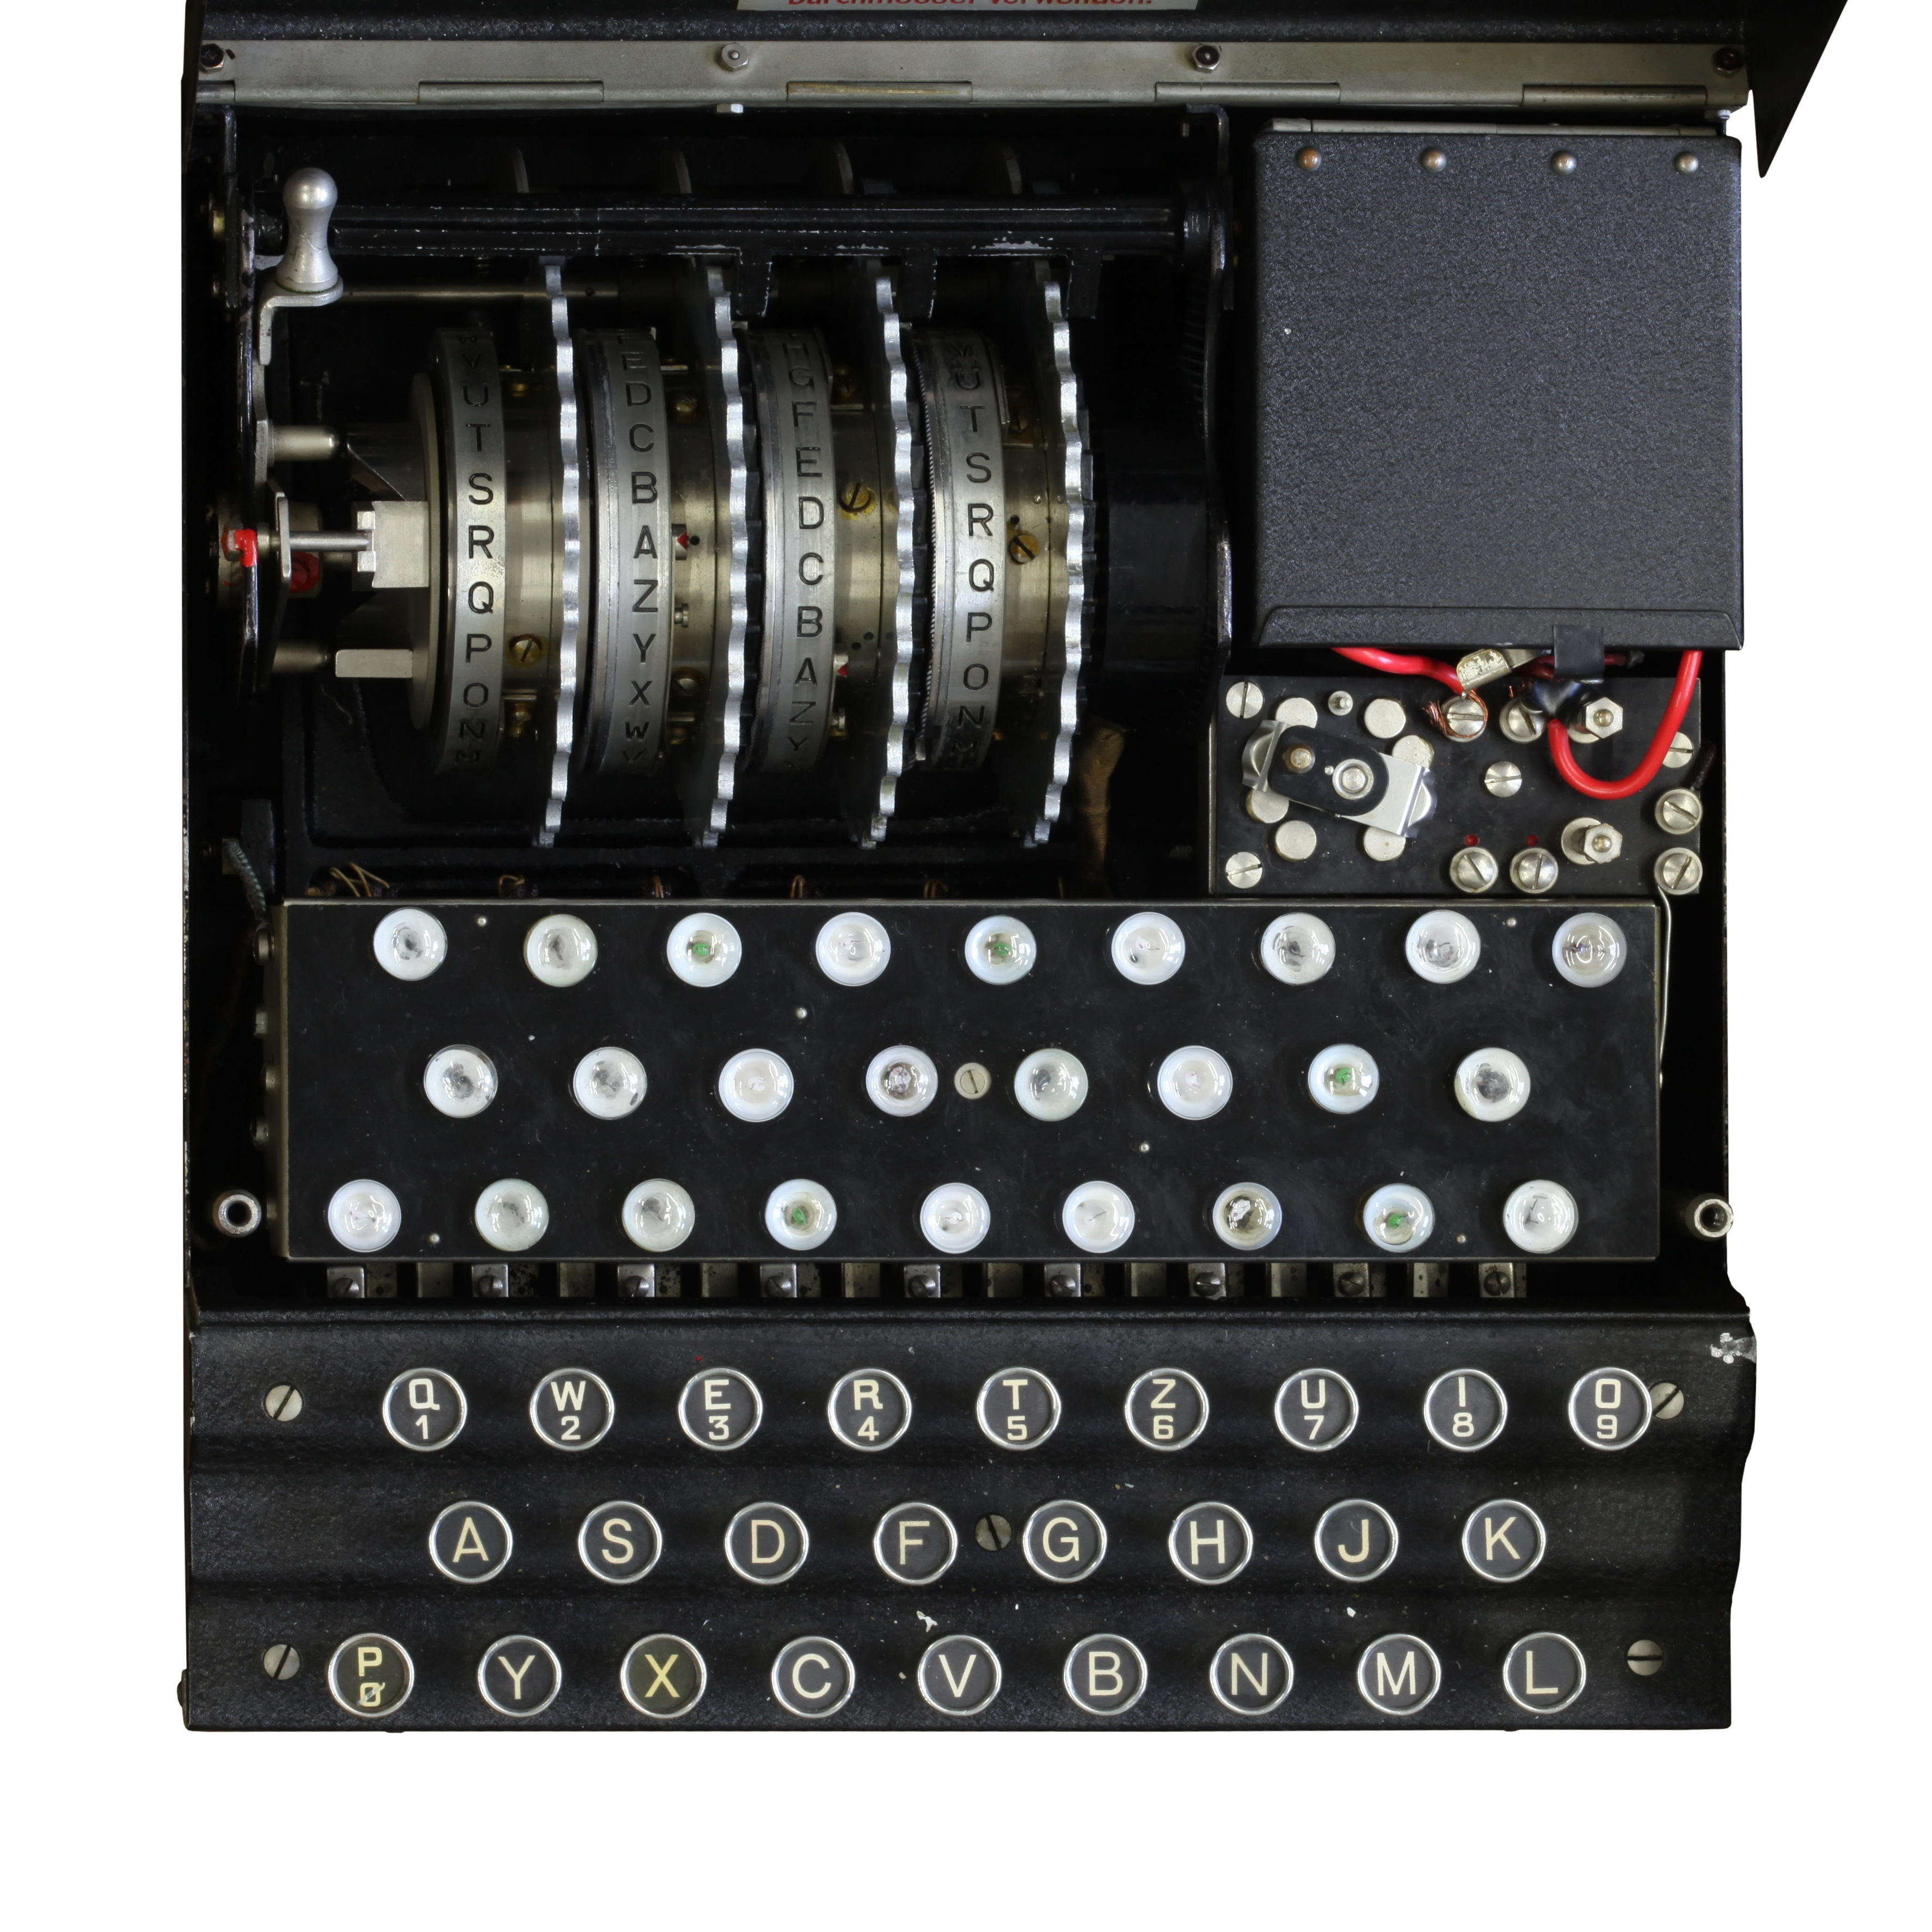
\includegraphics[height=10cm]{images/enigma.jpg}
  \caption{The Enigma Machine}
  \label{fig:machine1}
\end{centering}
\end{figure}

The first Enigma was shown in 1923 at the Universal Post Union Congress in Vienna. Germany soon after began to adopt the machines for military and government communications. They used the machines without much issue for many years. It wasn’t until 1930, with tensions remaining at a high level in Europe, that Poland felt the need to start protecting themselves, from Germany. They began intercepting German messages and attempting to decipher them. In the early 1930s, a member of the French General Staff, Capt. Gustave Betrand, took initiative to communicate with his opposite but equal peer in the Polish General Staff, after the French General Staff rejected a proposal by Poland to coordinate their intelligence gathering. Thanks to the direct communication between the men of different nations, intelligence gathered by France, particularly that which related to solving Enigma, was shared with Poland. Not the least of which was operating instructions and keying instructions of Enigma. We will see each of these documents come into play in the breaking of Enigma. The operating instructions helped the Polish Cipher Bureau determine the inner workings of the military Enigma machines. The keying instructions helped the cryptanalysts understand how the messages they were intercepting were structured. In early 1933 the Polish Cipher Bureau team had deduced the inner workings of Enigma and has commissioned the building of fifteen duplicates. Duplicating the machine, however, was not enough as the machines had to be given the correct settings to decipher a message correctly. These settings were, the public key that had to be transmitted with cipher text. At first they were simply found by process of elimination. In 1934 a member of the Polish Cipher Bureau team, Rejewski, made the cyclometer, which allowed the team to create a catalog of characteristics from the over 100,00 settings \cite{rfc01}. This made it much easier to find a key based on a given ciphertext, because a cryptanalyst could compare it with the cataloged characteristics. The cyclometer along with several other tools and practices, enabled the team to successfully decipher messages for over 5 years. 

In 1938, Germany made an effort to increase the complexity and security of their system by changing the keying practices, allowing for rotors to be placed in various slots, and other small changes to their enciphering practices. At the same time, the Polish Cipher Bureau team had made strides toward further automating the discovery of message keys. The Cryptological Bomb, or Bomba, was an electromechanical machine that in under 2 hours, would iterate over seventeen-thousand possibilities, stopping automatically when the desired one was found, and would turn on an indicator light. Also around this time, Germany began to occupy its neighboring nations, beginning with Austria. Throwing European politics into chaos, Britain and France were both looking for an ally with which to align themselves. Poland arose as the choice, and shortly before Germany’s occupation of Poland in late 1939, there had been a meeting of the three nations where Poland’s accomplishments were shared along with a great number of documents and resources, including one of the duplicate Enigma machines. As soon as the German forces made way into Poland, all work and remnants of the work done by the Cipher Bureau was destroyed, as the team of cryptanalysts fled to France. Before the end of the year, Britain had established Bletchley Park, the campus where the Ultra team would work to continue what the Polish Cipher Bureau had started. By all definitions, the Polish broke Enigma, and the British capitalized on their given knowledge to find solutions in record time \cite{rfc01}. Both extremely important to wartime intelligence. The British Bomb, or Bombe, was developed by Alan Turing who began work on the machine just after Britain’s first meeting with Poland and France. It accomplished the same task of the Bomba, determine the keyspace for a given ciphertext, but the Bombe looked at the entire text rather than just the encrypted settings at the beginning of the message. This enabled the machine to find a solution in 20 minutes rather than 2 hours. The accomplishments of each nation held great significance in the War and the efforts towards bringing it to an end.
    \chapter{Background}\label{chap:background}

The following will provide an introduction into some of the core concepts necessary to understand how Polish cryptologists were able to break Enigma in 1932. We will introduce the hardware of the Enigma machine, as well as provide a brief overview of permutation theory. We will also prove a theorem which is integral in creating the permutations used in the set of equations that model the electrical circuit inside Enigma.

\section{Enigma Hardware}

\begin{figure}[h!]
\begin{centering}
  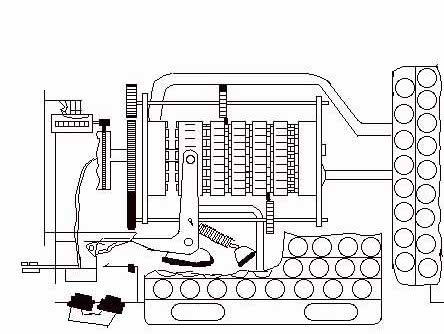
\includegraphics[height=8cm]{images/rotors.jpg}
  \caption{Hardware of the Enigma Machine}
  \label{fig:hardware1}
\end{centering}
\end{figure}

In order to understand how the ciphertexts created by the Enigma machine were broken, it is important to understand the inner workings of the machine itself. Figure \ref{fig:hardware1} shows a schematic of the hardware.

On the outside of each machine, there is a keyboard and a row of glowlamps. Each key on the keyboard is connected to a glowlamp through a changing electric circuit, so when a key is pressed it lights up a corresponding glowlamp. Below the keyboard, there is a plugboard with between six (6) and twelve (12) switches. These switches allow for two letters of the alphabet to be transposed prior to being sent into the machine's hardware. It introduced a "reciprocal monoalphabetic substitution between the keyboard and the first rotor" \cite{bw05}. This adds a layer of security beyond the rotors on the inside of the machine.

Inside each machine, there are anywhere from three (3) to as many as eight (8) rotors and a reflector, also known as a reversing drum. These rotors are the main ciphering components. Each rotor has the alphabet inscribed on the rim, twenty-six (26) fixed contacts on one face, and twenty-six (26) spring loaded contacts on the other face \cite{wk85}. Each rotor has a unique circumference, as well as a unique set of connected contacts. These contacts are randomly connected, and are different on each rotor \cite{bw05}. The reversing drum is responsible for creating the reciprocal nature of the machine, meaning that if an 'A' is pressed on the keyboard and an 'F' lights up on the glow lamps, it also means that if an 'F' is pressed on the keyboard, the 'A' will light up on the glow lamps.

Each rotor inside the machine is set up in such a way that it will rotate corresponding to different key presses. The rotor closest to the keyboard rotates every time a key is pressed, meaning that the substitution changes every time a key is pressed. The other two (2) to seven (7) rotors rotate at variable rates, depending on how the hardware is configured. The second rotor's rotation is dependent on the first rotor's rotation, the third rotor is dependent on the second, and so on and so forth. This rotation of the rotors adds another level of complexity on top of the already complex substitution cipher that Enigma creates.

\section{Important Mathematical Concepts}\label{sec:mathconcepts}

To understand some of the mathematical theory later on in this paper, one must first understand some basics of permutation groups. A permutation is a rearrangement of elements in a set. An example of this kind of permutation is rearranging the numbers ${1,2,3,4,5}$ into ${3,5,4,2,1}$. This could be expressed in the standard matrix form
$P = \begin{pmatrix}
    1 & 2 & 3 & 4 & 5 \\
    3 & 5 & 4 & 2 & 1
  \end{pmatrix}$, or in cyclic notation as $P_c = (1 3 4 2 5)$. Notice in cyclic notation that there is an implied transposition from $5$ to $1$ from the last element in $P_c$.

Permutations can be multiplied as well. In multiplying permutations, order is important. If we have
$$P = \begin{pmatrix}
    1 & 2 & 3 & 4 & 5 \\
    3 & 5 & 4 & 2 & 1
  \end{pmatrix}$$

$$Q = \begin{pmatrix}
    1 & 2 & 3 & 4 & 5 \\
    2 & 1 & 4 & 3 & 5
  \end{pmatrix}$$

One can multiply

$$QP = \begin{pmatrix}
    1 & 2 & 3 & 4 & 5 \\
    2 & 1 & 4 & 3 & 5
  \end{pmatrix}
  \begin{pmatrix}
    1 & 2 & 3 & 4 & 5 \\
    3 & 5 & 4 & 2 & 1
  \end{pmatrix}$$

To multiply, rearrange the columns of the $Q$ permutation (leftmost) so that the first row matches the $P$ permutation (or the rightmost). Then, take the non-matching rows of $P$ and $Q$ as the product. In this example, we get

$$QP = \begin{pmatrix}
    1 & 2 & 3 & 4 & 5 \\
    2 & 1 & 4 & 3 & 5
  \end{pmatrix}
  \begin{pmatrix}
    1 & 2 & 3 & 4 & 5 \\
    3 & 5 & 4 & 2 & 1
  \end{pmatrix} =
  \begin{pmatrix}
    3 & 5 & 4 & 2 & 1 \\
    4 & 5 & 3 & 1 & 2
  \end{pmatrix}
  \begin{pmatrix}
    1 & 2 & 3 & 4 & 5 \\
    3 & 5 & 4 & 2 & 1
  \end{pmatrix} =
  \begin{pmatrix}
    1 & 2 & 3 & 4 & 5 \\
    4 & 5 & 3 & 1 & 2
  \end{pmatrix}
  $$

In cyclic notation, $QP = (1 4)(2 5)(3)$.
\\

Another important concept necessary in order to fully understand the theory behind cracking the Enigma machine cipher is the \textit{Theorem on the Product of Transpositions}. A transposition is a 2-cycle permutation, for example $P = (13)$. A group of disjunctive transpositions, then, is a group of non-overlapping 2-cycles.
\\

The Theorem on the Product of Transpositions states that:
\\

\textit{If two permutations of the same degree consist solely of disjunctive transpositions, then their product will include disjunctive cycles of the same lengths in even numbers.}
\\

The proof is as follows:
\\

We assign two permutations to be multiplied to be $X$ and $Y$, with total degree $2n$. If both $X$ and $Y$ have identical transpositions within them, such as $(ab)$, then the product will have two distinct cycles $(a)$ and $(b)$. This makes up our base case, as any two permutations with identical transpositions will have an even number of disjunctive transpositions.

Our next step occurs as such. If permutation $X$ includes a transposition $(a_1 a_2)$, there must be a permutation in $Y$ that begins with $a_2$, such as $(a_2 a_3)$. We have already ruled out the possibility of $Y$ including $(a_2 a_1)$ in our base case. We can continue this logic and say the following:

$$(a_1 a_2), (a_3 a_4), ..., (a_{2k-3} a_{2k-2}), (a_{2k-1} a_{2k}) \in X$$
$$(a_2 a_3), (a_4 a_5), ..., (a_{2k-2} a_{2k-1}), (a_{2k} a_{1}) \in Y$$

From these two sets $X$ and $Y$, when we multiply them together we will always obtain two cycles of the same length $k \leq n$:

$$(a_1 a_3 ... a_{2k-3} a_{2k-1}) (a_{2k} a_{2k-2} ... a_4 a_2)$$

We continue this step until there are no more elements in $X$ and $Y$, with the result that the product will only include disjunctive cycles of the same lengths in even numbers, which concludes the proof. This proof was adapted from Appendix E from Kozaczuk \cite{wk85}.

In the breaking of Enigma, Polish mathematicians also used the converse of the above proof, which states that \textit{if a permutation of even-numbered degree includes disjunctive cycles of the same lengths in even numbers, then this permutation may be regarded as a product of two permutations, each consisting solely of disjunctive transpositions}.

    \chapter{Examples}\label{chap:examples}

\section{Encryption Process}

In accordance with Kerchoff's principle, the method of encrypting a message was known by the Polish and British cryptologists attempting to break the cipher. In this paper, we will touch on two (2) separate methods of encrypting a message that were used during World War II. The first method was common practice until September 1938, when Germany decided to increase security by changing to the second method, which was used from then on.

\section{Encryption Process Pre-1938}\label{sec:encprocess1938}

Prior to the security changes in 1938, the process for encryption stayed mostly static. The encipherer, person who wanted to encrypt a message, would begin by setting their machine to the daily settings found in the widely dispersed codebook, say "JEF". These daily settings would correspond to initial settings of the rotors (which alphabetic character was visible from the top of the machine), as well as the settings of the plugboard (which letters would be transposed with which other letters). From there, the encipherer would choose their own individual key, which was supposed to be a random set of three (3) characters that was unique to the individual message, say "KCB". They would type their individual key into the Enigma machine twice, "KCBKCB" thus encrypting it twice using the daily settings, resulting in 6 distinct characters "BQROMP". They typed it twice so as to ensure that there were no errors in encrypting the key, similar to how websites ask for a password confirmation on creation of a password. After encrypting the password using the daily settings, the encipherer would set the machine to their individual key, "KCB" and encrypt the actual message. \cite{wt06}. The six indicator letters would sit as a preamble to the rest of the message. 

In order to decipher the message received, the decipherer would follow an almost identical process. They would set their machine to the daily key, and type the first six (6) letters of the message, "BQROMP", into the machine. This would reveal the individual key, "KCB". After ensuring that it was error-free, the decipherer would set their machine to the individual key, and type in the rest of the message to reveal the plain text. Note that the same machine (the same internal hardware) is used to both encrypt and decrypt the message.

\section{Mathematical Theory Behind Cracking Enigma}

The initial goal in cracking the Enigma machine was to determine the hardware connections on the rotor closest to the keyboard. Knowing the hardware connections on that rotor would allow the Polish mathematicians to reconstruct their own Enigma machine, and use that to decrypt more messages. It would open the doors for more rapid and widespread decryption.

Of course, it was not easy to find out what the hardware connections on the rotor were. All the mathematicians had to work with were ciphertexts that had been intercepted throughout the day, so they could only attempt ciphertext-only attacks. However, Polish mathematicians Marian Rejewski, Jerzy Rozycki, and Henryk Zygalski were able to crack the Enigma cipher in 1932. The solution to this believed 'impossible' problem took its roots in the permutation theory that was covered in \secref{sec:mathconcepts}, with some help from the enciphering process itself, covered in \secref{sec:encprocess1938}.

Since every message was encrypted with a different individual key, coupled with the fact that each rotor rotated at different speeds, it was impossible to determine the plain text just by comparing ciphertexts. However, with knowledge of the encryption process, it was possible to draw conclusions about the first six (6) letters of each ciphertext, and with enough ciphertexts, draw conclusions about the inner workings of the Enigma machine. The mathematicians knew that the first six (6) letters were a repeat of the same three (3) letter key, they could draw two conclusions.

\begin{enumerate}
\item All message keys started from the same position, set from a codebook.
\item The first letter in the plaintext was the same as the fourth, the second the same as the fifth, and the third the same as the sixth.
\end{enumerate}

This is where permutation theory comes in. In this section of the paper, we will make reference to permutations $A$ - $F$, which correspond in kind to a different substitution cipher created by Enigma. $A$ corresponds to the transposition of letters (of the form $(ab)(cd)(ef)...$ where each letter occurs once) that occurs on the very first keypress in an encryption, which correlates to the first value in the encipherer's individual key. $B$ then corresponds to the transposition that occurs on the second keypress, $C$ on the third, and so on. One will notice that $A$ and $D$ both correspond to the first value in the encipherer's individual key, $B$ and $E$ correspond to the second, and $C$ and $F$ correspond to the third. This was one of the first conclusions drawn by the Polish mathematicians as well.

The first step to cracking Enigma involved gathering as many ciphertexts as possible and recognizing products of permutations within them. We know that $A$ and $D$ correspond to the same letter. This means that when the encipherer types a character $x$, he obtains the value $a$ as his ciphertext, and when he types the same character $x$ for the double enciphering of his individual key (in the fourth place), he obtains the value $b$, indicating a relationship between the values $a$ and $b$. This relationship between keys here can be modeled as a product of permutations $AD$, which is the product of the individual permutations $A$ and $D$.

As an example, take the ciphertexts

\begin{CVerbatim}[fontsize=\small]
dmq vbn
von puy
puc fmq
\end{CVerbatim}

One can see that $d \rightarrow v$, $v \rightarrow p$, and $p \rightarrow f$. That means that the permutation $AD$ contains $dvpf$. The same process can be applied to see that $oumb$ is in $BE$ and $cqny$ is in $CF$. If enough ciphertexts are gathered such that each letter of the alphabet is seen in each position at least once, entire permutations can be constructed. The permutation sets created from the daily ciphertexts are called the 'characteristic' for the day \cite{wk85}.

\begin{figure}[h!]
\begin{centering}
  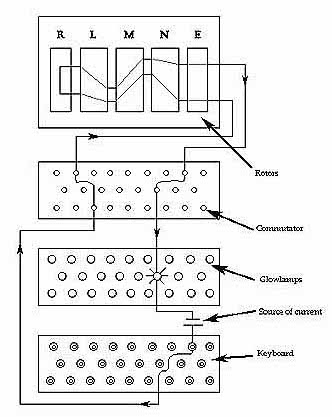
\includegraphics[height=10cm]{images/permutations.jpg}
  \caption{Electric Current Through Enigma}
  \label{fig:current1}
\end{centering}
\end{figure}

Next, it is important to understand how the machine works, with regards to a circuit. \figref{fig:current1} shows the circuit that is created when a key is pressed. If we label the commutator (or plugboard) as $S$, the three rotors from left to right as $L$, $M$, $N$ respectively, and the reversing drum $R$, we can represent the path of the current as the product of the permutations $SNMLRL^{-1}M^{-1}N^{-1}S^{-1}$. However, we also need to account for the fact that the $N$ rotor revolving $1/26th$ of a turn each time a key is pressed, and we can represent that with the permutation $P = (abcdefghijklmnopqrstuvwxyz)$. Thus, if the $N$ rotor rotates twice, we will have $P^2$, and so on and so forth. With this, we can rewrite the previous equation for each individual keypress, including $P$.

$$A = SPNP^{-1}MLRL^{-1}M^{-1}PN^{-1}P^{-1}S^{-1}$$
$$B = SP^2NP^{-2}MLRL^{-1}M^{-1}P^2N^{-1}P^{-2}S^{-1}$$
$$C = SP^3NP^{-3}MLRL^{-1}M^{-1}P^3N^{-1}P^{-3}S^{-1}$$
$$D = SP^4NP^{-4}MLRL^{-1}M^{-1}P^4N^{-1}P^{-4}S^{-1}$$
$$E = SP^5NP^{-5}MLRL^{-1}M^{-1}P^5N^{-1}P^{-5}S^{-1}$$
$$F = SP^6NP^{-6}MLRL^{-1}M^{-1}P^6N^{-1}P^{-6}S^{-1}$$

It is clear that $MLRL^{-1}M^{-1}$ is repeated in every one of these equations, so we can replace that value with the value $Q$. \cite{wk85} We also must calculate the products $AD$, $BE$, and $CF$ with respect to the above equations, and we get the following equations:

$$AD = SPNP^{-1}QPN^{-1}P^3NP^{-4}QP^4N^{-1}P^{-4}S^{-1}$$
$$BE = SP^2NP^{-2}QP^2N^{-1}P^3NP^{-5}QP^5N^{-1}P^{-5}S^{-1}$$
$$CF = SP^3NP^{-3}QP^3N^{-1}P^3NP^{-6}QP^6N^{-1}P^{-6}S^{-1}$$

In order to solve these equations, we can take one of two routes. One, we can solve for $S$, $N$, and $Q$ using $AD$, $BE$, and $CF$. Two, we can solve for $A$ - $F$, $S$, $Q$, and $N$. One may notice that there are more unknowns than equations, which makes these sets impossible to solve. This is where the Polish mathematicians hit a stopping point. That is, until the French Cipher Bureau was able to provide the Polish Cipher Bureau with some codebooks that they had recovered from the Germans \cite{wk85}. This gave the Polish mathematicians the values of $S$ that they needed. They were also able to determine $A$ - $F$ based on encipherer's habits, and applications of the converse Theorem on the Product of Transpositions discussed in \secref{sec:mathconcepts}. Therefore, the four (4) unknowns from the equations was reduced to two (2), which is solvable.

$$SAS^{-1} = PNP^{-1}QPN^{-1}P^{-1}$$
$$SBS^{-1} = P^2NP^{-2}QP^2N^{-1}P^{-2}$$
$$SCS^{-1} = P^3NP^{-3}QP^3N^{-1}P^{-3}$$
$$SDS^{-1} = P^4NP^{-4}QP^4N^{-1}P^{-4}$$
$$SES^{-1} = P^5NP^{-5}QP^5N^{-1}P^{-5}$$
$$SFS^{-1} = P^6NP^{-6}QP^6N^{-1}P^{-6}$$

$N$ and $Q$ were able to be solved using the known values, and the resulting $N$ permutation corresponded to the connectors in that specific rotor \cite{wk85}. That $N$ was the result the mathematicians were after, and it was this permutation that was integral to continuous decryption of messages throughout the 1930s.

\section{Encryption Process Post-1938}

Germany realized that their messages were being successfully intercepted, and to throw off their enemies, added some complexities to the Enigma machines and the practices of using it. First, they added two rotors to the existing three. This increased the combination of rotor positions from 6 to 60. Previously, the Poles had 6 Bomby, one for each possible position, that would iterate over rotation settings for the given position, in an effort to find the keys to messages of the day. The increase in hardware complexity rendered this method essentially obsolete. Also recognizing the fault in double-enciphering message keys, they replaced the practice. Rather than starting with a network-wide common setting, clerks would choose three random letters, say "WER", and use this as their initial setting. Choosing three more random letters still, "IUY", the clerk would encrypt this indicator only once, giving "BSD". The new preambles would be comprised of the initial setting, followed by the encrypted indicator, "WERBSD". This troubled the Ultra team at Bletchley Park for a time, until they began to find patterns and habits in the clerks' use of the machines. They were lazy and would use letter combinations that did not require much thought: repeating letters, ones that sat next to each other on the keyboard, or names. Sometimes the clerks would not change the settings between messages at all and would simply use the ending state of their machine from one message as the beginning stage for a new one \cite{mf01}. These habits, dubbed "cillies" by Bletchley Park, are what allowed the team to reframe their approach to deciphering messgaes. 

\section{Cryptological Machines}



    \chapter{Conclusion}\label{chap:conclusion}

When Germany caught wind of the fact that Enigma could be broken, they attempted different methods to increase security, such as changing the way the key was created, or changing the rotor arrangement \cite{wk85}. Each of these attempts at increasing security only set the Poles back a week or so at most, and soon they were back to being able to crack the codes just as they were before. In fact, when the Germans changed the rotor arrangement, it actually helped the Polish mathematicians. Moving the known $N$ rotor to another position meant that they already knew the connections of that rotor, and then they could use the same method as before to figure out the new rotor that was closest to the keyboard. This simple mistake by Germany, coupled with the habits of the encipherers when creating their individual keys, brings to the forefront an idea that is important to grasp from this paper. Enigma would have been unbreakable if it had not been for the encipherers' habits and predictability. Human error was the only real issue with the cryptosystem. This is the case for many cryptosystems: they are theoretically incredibly secure, but in practice are misused. It would be easy to blame Germany's lack of training the encipherers on the reason there were so many habitual individual keys, but that would be naive. Humans are as a rule habitual beings, and so it would be interesting to try to create a cryptosystem that completely erases human vulnerability.

To conclude, Enigma was an incredible asset to the Germans during World War Two, and was an even greater asset to the Allies when they were able to crack it. It was also a large step in cryptological machines, as it was one of the first widely believed 'unbreakable' cipher machines in existence. The machine spurred new technological advancements such as the cryptological bombes, including the one created by Alan Turing. Without this cryptological machine, we might not be where we are today with regards to technology, so we have that to thank for it.

    % bibliography is not in the table of contents per default, add it manually
    \addcontentsline{toc}{chapter}{Bibliography}
    \bibliographystyle{ieeetr}
    \bibliography{bib/topic1}
    \newpage
    \thispagestyle{empty}
    \mbox{}


\end{document}
